% Part: model-theory
% Chapter: interpolation
% Section: separation

\documentclass[../../../include/open-logic-section]{subfiles}

\begin{document}

\olfileid{mod}{int}{sep}

\olsection{\printtoken{P}{sentence} चे विलगीकरण}

अंतर्वेशन प्रमेयाची सिद्धता सुरू करण्यापूर्वी थोडी पूर्वतयारी आवश्यक आहे.
$!A$ आणि~$!B$ यांचे अंतर्वेशक म्हणजे असे !!a{sentence}~$!C$ की
$!A \Entails !C$ आणि $!C \Entails !B$. प्रतिपरिवर्तनानुसार, यांपैकी
नंतरचे विधान तेव्हा आणि केवळ तेव्हाच खरे असते, जेव्हा $\lnot !B
\Entails \lnot !C$. हा गुणधर्म असलेले !!^a{sentence}~$!C$ हे $!A$
आणि~$\lnot !B$ यांना \emph{विलग करते} असे म्हणतात. म्हणून $!A$ आणि~$!B$
यांचे अंतर्वेशक शोधणे म्हणजे $!A$ आणि~$\lnot !B$ यांना विलग करणारे
!!a{sentence} शोधणेच होय. नेहमीप्रमाणे, याचे व्यापक रूप विचारात घेणे उपयोगी
ठरेल: !!{sentence}s च्या दोन \emph{संचांना} विलग करणारे वाक्य.

\begin{defn}
वाक्य~$!C$ हे वाक्यसंच~$\Gamma$ आणि~$\Delta$ यांना \emph{विलग करते}
तेव्हा आणि केवळ तेव्हाच, जेव्हा $\Gamma \Entails !C$ आणि $\Delta
\Entails \lnot !C$. असे कोणतेही !!{sentence} अस्तित्वात नसेल, तर
$\Gamma$ आणि~$\Delta$ यांना \emph{अविलगनीय} म्हणतात.
\end{defn}

$\Gamma$, $\Delta$ आणि~$!C$ यांच्या प्रतिमान-वर्गांमधील समावेशन-संबंध
खाली दर्शवले आहेत:
\begin{figure}[h]
  \centering
  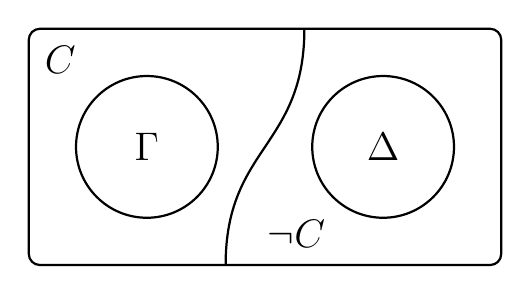
\begin{tikzpicture}[node distance=2cm, auto, thick]
    \draw [rounded corners] (0,0) -- (6,0) -- (6,3) -- (0,3) --  cycle;
    \draw (1.5,1.5) circle (0.9cm);
    \draw (4.5,1.5) circle (0.9cm);
    \path node at (1.5,1.5) {\Large $\Gamma$};
    \path node at (4.5,1.5) {\Large $\Delta$};
    \path node at (0.4,2.6) {\Large $\formula{C}$};
    \path node at (3.4,0.4) {\Large $\lnot \formula{C}$};
    \draw (2.5,0) .. controls (2.5,1.5) and (3.5,1.5) .. (3.5,3);
  \end{tikzpicture}
  \caption{$!C$ हे $\Gamma$ आणि $\Delta$ यांना विलग करते}
  \ollabel{fig:sep}
\end{figure}


\begin{lem}\ollabel{lem:sep1}
समजा $\Lang{L}_0$ या भाषेत $\Gamma$ आणि~$\Delta$ या \emph{दोन्हींमध्ये}
आढळणारे प्रत्येक !!{constant}, !!{function} आणि !!{predicate} ($\doteq$
खेरीज) येते; आणि प्रत्येक $n \ge 0$ साठी अनंत नवीन !!{constant}s
$\Obj c_n$ जोडून $\Lang{L}'_0$ मिळवली आहे. मग $\Gamma$ आणि~$\Delta$ हे
$\Lang{L}_0$ मध्ये अविलगनीय असतील, तर ते $\Lang{L}'_0$ मध्येही अविलगनीय
असतात.
\end{lem}

\begin{proof}
विरोधाभास पद्धतीने सिद्ध करू: विरुद्धार्थी असे समजा की $\Gamma$ आणि
$\Delta$ हे $\Lang{L}'_0$ मध्ये विलगनीय आहेत. मग एखाद्या $!C \in
\Lang{L}_0$ साठी $\Gamma \Entails \Subst{!C}{c}{x}$ आणि $\Delta
\Entails \lnot \Subst{!C}{c}{x}$ असते (येथे $c$ हे नवीन !!{constant}
आहे---$!C$ मध्ये अशी एकाहून अधिक नवीन !!{constant} असलेले प्रकरणही यासारखेच
आहे). संहततेनुसार, $\Gamma$ चा \emph{सांत} उपसंच~$\Gamma_0$ आणि
$\Delta$ चा सांत उपसंच~$\Delta_0$ असे आहेत की $\Gamma_0 \Entails
\Subst{!C}{c}{x}$ आणि $\Delta_0 \Entails \lnot \Subst{!C}{c}{x}$.
$\Gamma_0$ मधील सर्व !!{formula}s चा संयोग~$!G$ आणि $\Delta_0$ मधील सर्व
!!{formula}s चा संयोग~$!H$ असू द्या. मग
\begin{align*}
  !G & \Entails \Subst{!C}{c}{x}, & !H  \Entails \lnot \Subst{!C}{c}{x}.
\end{align*}
पहिल्या विधानावर सामान्यीकरण लावल्यास $!G \Entails \lforall[x][!C]$
मिळते; आणि दुसऱ्यावर प्रतिपरिवर्तन लावल्यास $\Subst{!C}{c}{x}
\Entails \lnot !H$ मिळते, म्हणून $\lforall[x][!C] \Entails \lnot !H$.
%READERNOTE{OLFOL-041 — गोठवलेल्या इंग्रजीतील या निष्पन्नतेच्या उजव्या बाजूस आधी परिभाषित केलेल्या H ऐवजी असंबद्ध ग्रीक डेल्टा छापले आहे. पुढील वाक्यातील प्रतिपरिवर्तनासाठी आणि संपूर्ण युक्तिवादासाठी येथे H चाच निषेध आवश्यक आहे; मराठी सूत्रात H पुनःस्थापित केला आहे.}
पुन्हा प्रतिपरिवर्तन केल्यास $!H \Entails \lnot \lforall[x][!C]$
मिळते. एकस्वनिकतेनुसार,
\begin{align*}
  \Gamma &\Entails \lforall[x][!C], &
  \Delta & \Entails \lnot \lforall[x][!C],
\end{align*}
त्यामुळे $\lforall[x][!C]$ हे $\Lang{L}_0$ मध्ये $\Gamma$ आणि~$\Delta$
यांना विलग करते.
\end{proof}

\begin{lem}\ollabel{lem:sep2}
समजा $\Gamma \cup \{ \lexists[x][!S] \}$ आणि~$\Delta$ हे अविलगनीय
आहेत, आणि $c$ हे $\Gamma$, $\Delta$ किंवा~$!S$ यांपैकी कशातही नसलेले नवीन
!!{constant} आहे. मग $\Gamma \cup \{ \lexists[x][!S],
\Subst{!S}{c}{x} \}$ आणि~$\Delta$ हेही अविलगनीय असतात.
\end{lem}

\begin{proof}
विरोधाभासासाठी असे समजा की $!C$ हे $\Gamma \cup \{ \lexists[x][!S],
\Subst{!S}{c}{x}\}$ आणि~$\Delta$ यांना विलग करते, पण त्याच वेळी
$\Gamma \cup \{\lexists[x]{!S} \}$ आणि~$\Delta$ हे अविलगनीय आहेत. दोन
प्रकरणे वेगळी करू:
\begin{enumerate}
\item $!C$ मध्ये $c$ आढळत नाही: या प्रकरणात $\Gamma \cup
  \{\lexists[x][!S], \lnot!C \}$ हा संच पूर्ततायोग्य असतो (अन्यथा
  $!C$ हे $\Gamma \cup \{\lexists[x][!S] \}$ आणि~$\Delta$ यांना विलग
  करेल). $\Subst{!S}{c}{x}$ ची भर घातल्यानंतरही तो पूर्ततायोग्य राहतो;
  म्हणून अखेरीस $!C$ हे $\Gamma \cup \{ \lexists[x][!S],
  \Subst{!S}{c}{x} \}$ आणि~$\Delta$ यांना विलग करत नाही.
\item $!C$ मध्ये $c$ आढळते, त्यामुळे $!C$ चे रूप
  $\Subst{!C}{c}{x}$ असते. मग
  \[
  \Gamma \cup \{ \lexists[x][!S], \Subst{!S}{c}{x}\} \Entails \Subst{!C}{c}{x},
  \]
  असे असते. यावरून निगमन प्रमेय आणि सामान्यीकरण यांच्या साहाय्याने
  $\Gamma, \lexists[x][!S] \Entails \lforall[x][(!S \lif !C)]$ आणि
  अखेरीस $\Gamma \cup \{ \lexists[x][!S] \} \Entails
  \lexists[x][!C]$ मिळते. दुसरीकडे, $\Delta \Entails \lnot
  \Subst{!C}{c}{x}$; म्हणून सामान्यीकरणाने $\Delta \Entails \lnot
  \lexists[x][!C]$. त्यामुळे $\Gamma \cup \{\lexists[x][!S] \}$
  आणि~$\Delta$ हे विलगनीय ठरतात, आणि हा विरोधाभास आहे.
\end{enumerate}
\end{proof}

\end{document}
